\documentclass[11pt]{article}
\usepackage{todonotes}
\usepackage{float}
\usepackage{caption}
\usepackage{subcaption}
\usepackage[backend=biber,style=authoryear,url=false]{biblatex}
%\bibliography{bibevol2.bib}
\bibliography{bibevol.bib}
%\bibliography{bibevol3.bib}
\bibliography{bibevol4.bib}
\usepackage{sgame}
\usepackage{tikz}
\usepackage{pgfplots}
 % Useful for Physics related math
\usepackage{physics}
\usepackage{amsmath}
\usepackage{amssymb} 
\usepackage{amsthm}
        % packages that allow mathematical formatting
\usepackage{setspace}
\setlength\parindent{0pt}
        % set space and indent and indent
\usepackage{hyperref}
\hypersetup{
            colorlinks,
                linkcolor={red!50!black},
                    citecolor={blue!50!black},
                        urlcolor={blue!80!black}
                }
\usepackage[a4paper,width=150mm,top=25mm,bottom=25mm]{geometry}

% New commands
\let\conju\overline
\newcommand\numberthis{\addtocounter{equation}{1}\tag{\theequation}}
\newcount\colveccount
\newcommand*\colvec[1]{
        \global\colveccount#1
        \begin{pmatrix}
                \colvecnext
        }
        \def\colvecnext#1{
                #1
                \global\advance\colveccount-1
                \ifnum\colveccount>0
                \\
                \expandafter\colvecnext
                \else
        \end{pmatrix}
        \fi
}
        % Columnvectors
\newtheorem{mydef}{Definition}

\pgfplotsset{compat=1.11}
\linespread{1.5}
\newcommand{\natnumb}{\mathbb{N}}
\newcommand{\realnumb}{\mathbb{R}}
\presetkeys{todonotes}{color=yellow,size=\scriptsize}{}
\begin{document}
\section{Introduction}

The beginnings of game theory date back to Johann von Neumann in 1928 
\parencite{v._neumann_zur_1928}, who developed a mathematical framework
for modelling situations with strategic interactions of rational agents.
In a situation of strategic interaction, the outcome for an agent does not
only depend on his choice, but also on the choice of the other agents.
In economics, such situations often present themselves as a social dilemma,
a situation where a group of agents is prevented to achieve the best
outcome for the group, because of strategic considerations of the individual
agent.
Asking a social scientists about \textit{the} example of a social dilemma, 
one usually gets to hear the story about two prisoners, arrested and 
seperately interrogated by an authority. Lacking the amount of evidence to sue 
the criminals for serious crimes, the authority offers them a deal 
simultaneously.
A confession grants a prisoner with amnesty and hence he escapes the punishment
for the serious crimes. However, if both choose to confess, they receive the
full sharpness of the law. Not admitting the crimes would leave the authority
with too little evidence, resulting only in a sentence for minor crimes.
This story, developed by Albert Tucker in 1950 and suitably named Prisoner's
Dilemma(PD) is usually represented in a table, as shown in figure \ref{fig:pd}, with
the options for each prisoners denoted by C, remaining silent, and D, admiting
their crimes. The dilemma is that the total amount of years for the group
is lowest if both do not confess, but each individual prisoner has the 
incentive to take the deal of the authority as this leaves him, independently
of what his fellow prisoner does, with a lower time in prison. Hence, 
individual interest and the benefit of the group are in conflict
\parencite{skyrms_stag_2004}. However, there is another "story that became
a game" \parencite[1]{skyrms_stag_2004}, which describes a different, but
as Skyrms argues, underrepresented social dilemma. In \textit{A Discourse on
Inequality}, Rousseau outlines the situation of hunters, heading out to hunt 
stag. However, if a hare runs past a hunter, he might consider to
shoot the hare, banishing all stags in the forest. The total reward for
the group is surely lower, but it is rationale for the single hunter if he
expects the others to act the same, given the opportunity. In contrast
to PD, it is not the hunters individual interest that is competing with the
benefit of the group, but the uncertainty about what the other hunters choose
to do. In fact, none of the hunters would have bad feelings about his choice
not to shoot a hare when returning with a stag, as his personal benefit is 
greater with a stag as bounty. Figure \ref{fig:sh} represents this dilemma 
for two hunters. When both coodinate on stag hunting, denoted by S, they receive 
$5$. If one of them decides to shoot the hare, he gets $4$, whereas
the other hunter is left out in the cold with no prey. Coordination on hare
hunting yields both $2$. In game theory, this type of situation is called
a coordination game. Since in the outcomes the hunters coordinated, either
on hunting stag or hare, they have no incentive to change their action. 
Both outcomes are what game theory calls a Nash-equilibrium, originally
formulated by John Nash in 1950 \parencite{nash_equilibrium_1950}. In a 
Nash equilibrium all players of a game choose a best reply against
the strategies of the other players, so that none of them has an incentive
to deviate unilateral from his decision. Although this is the mainly used
solution concept, it does not give a definite answer in the stag hunt game.
One might argue that both hunters can speak to each other beforehand and
assure each other that hare hunting is more attractive to both them. However,
\textcite{camerer_behavioral_2003} argues that empirical observation and theory 
suggest that the problem is not solved that easily.
Furthermore, in a wide range of economic applications interaction of agents
happen repeatedly. Analyzing repeated prisoner dilemmas, it turns 
out that the resulting game can actually be interpreted as a stag-hunt game with
two Nash equilibria \parencite{skyrms_stag_2004}.
This connection between this two social dilemmas advocates that
the selection of equilibria should be investigated more deeply. 
An interesting approach to the equilibrium selection problem comes from
biology. Evolutionary game theory was pioneered by Maynard J. Smith and George
R. Pricein their work on the conflict of animals in populations 
\parencite{smith_lhe_1973}. Started as a refinement of the Nash equilibrium,
the concept of an evolutionary stable strategy, various other authors, for 
example \textcite{taylor_evolutionary_1978}, \textcite{hofbauer_note_1979} and
\textcite{zeeman_dynamics_1981}, developed a "time dependent dynamical
extension of game theory" \parencite[55]{hanauske_evolutionare_2011}.
In contrast to traditional game theory, the evolutionary approach  models
 agents in a large population, interacting repeatedly in a strategic enviroment. 
Furthermore, the agents are not assumed to be rational, but follow a specific 
rule, updating their strategy. 
As outlined in the rest of this text, the
evolutionary approach offers an answer to the coordination problem in the
stag hunt game.

The thesis is organized as follows. Chapter 2 introduces the 
framework of traditional game theory for the stag hunt game and discusses
the traditional approach to the equilibrium selection problem. Chapter 3
motivates evolutionary game theory and presents the replicator dynamic. 
Later on, it will be discussed how the evolutionary approach selects
between multiple equilibria. Chapter 4 demonstrates the effect of a
network externality in the underlying framework. Looking for evidence
how real people play the stag hunt game, chapter 5 considers experimental
literature on the topic. Chapter 6 concludes and shows application of
evolutionary game theory and the stag hunt game in economics.

\begin{figure}[h]
\begin{center}
\begin{game}{2}{2} & $S$ & $H$
\\ $S$ &$5,5$ &$0,4$
\\ $H$ &$4,0$ &$2,2$ \end{game}
\label{sh}
\end{center}
\caption{A parametrized representation of the Stag hunt game, $a>c\geq d >b$}
\end{figure}
\begin{figure}[h]
\begin{center}
\begin{game}{2}{2} & $C$ & $D$
\\ $C$ &$-1,-1$ &$-4,0$
\\ $D$ &$0,-4$ &$-3,-3$ \end{game}
\end{center}
\label{pd}
\caption{A parametrized representation of the prisoners dilemma}
\end{figure}
\section{The Stag hunt game}
\label{sec:traditional}
\todo{Motivation of traditional game theory}
As introduced, the stag hunt game (SH) is played by two players who choose their
strategies without knowing each others choice.
Both have information about the strategies of the
other player and the payoffs they and their opponents receive. In game theory
such a game is called a \textit{normalform} game. Typically, such a game is
formalized as a Triplet $\Gamma = (I,\mathbb{S},F)$, with the set of players 
$I=\{1,2,...,n\}$, where $n$ is the total number of players.
The pure strategy space of the game $\mathbb{S} = \times_i S_i$
with the pure strategy space $S_i$ of an individual player 
$i \in I$ defined as $S_i = \{1,2,...,m_i\}$, where $m_i$ denotes the total
number of strategies available to player $i$. The payoff function of the game
is denoted by $F: S \rightarrow \realnumb^n$.
As this text focusses on the stag hunt game, this definitions reduce to the 
following.
By setting $n=2$, we define the set of two hunters playing SH as $I=\{1,2\}$. A 
player $i \in I$  can choose from a set of pure strategies from his 
pure strategy space, $S_i$. The strategies are called pure to distinguish
them between the later introduced mixed strategies. 
In the SH game, each hunter can choose one out of two pure strategies, namely, 
huntig the stag (strategy 1) or hunting hare (strategy 2).
Therefore, the pure strategy space is defined by $S_i = \{1,2\}$, which results
by setting $m_i=2$. In the SH game both players choose from
the same set of stragies such that $S_1 =S_2=S$. Combining the strategy spaces
of the two players with the cartesian product
yields the definition of the pure strategy space of the game
$\mathbb{S}= S \times S = S^2$. Games played by two players with two strategies
each, are often said to be \textit{2x2 games}.

In the analogy of the story Rousseau told, the hunters do not just hunt
for their pleasure, but to sell their loot for a reward. 
This is captured by the definition of an individual payoff function for player
i, $F_i:S \rightarrow \realnumb$, which maps a payoff $F_i(s) \in \realnumb$ 
to every state of the game $s=(s_1,s_2) \in S^2$, where $s_i$ i s a pure
strategy of player $i$.\todo{this sentence}
The payoffs are usually interpreted as \textit{Von-Neumann}-utility when 
played by individuals or households and represent earnings regarding firms. 

In the special case of two player, one 
can define a payoff matrix for player 1, $A \in \realnumb^{2 \times2}$ and for 
player 2,  $B \in \realnumb^{2 \times2}$, where $A_{kl} = F_1(k,l)$ and $
B_{kl} = F_2(k,l)$ with the pure strategies $k,l \in S$. Using the 
representation above, one can indentify the payoff matrices for the player as
\begin{align}
     A = \mqty(a && b \\ c && d), \quad B = \mqty(a && c \\ b && d)
        \label{eq:matrix}
\end{align}
For the game here in study, the following definition is important: 
\begin{mydef}
        A two player game $\Gamma=(I,S_1 \times S_2, A,B)$ is called symmetric
        if the players of the game have the same strategy space $S_1=S_2=S$ and
        for the payoff matrices the condition $B=A^T$ holds. Therefore, the
        game is well-defined as $\Gamma=(I,S^2,A)$.
        \label{symmetry}
\end{mydef}
Clearly, the SH game satisfies this condition. Both hunters have the same 
strategies available and the payoff matrices defined in 
\eqref{eq:matrix}  are the transpose of the other.
Hence, it is irrelevant which player is labeled as player 1 or 2, because 
they are identical with respect to their strategies and payoffs.

Usually a game is extended by the possibility of the players to play
\textit{mixed strategies}. 
The first intuition of a mixed strategy in the SH game would be hunters
choosing whether to shoot the stag or the hare by using a randomization
tool such as flipping a coin. However, randomization is not really
satisfying in the most applications \parencite{radner_private_1982}. An
alternative interpretation, outlined by Rubinstein, is that mixed 
strategies are actually deterministic, but seem to be random because they 
depend on not modelled private information of the individuals 
\parencite[914]{rubinstein_comments_1991}. In the evolutionary context
discussed in section \ref{evolutionarystaghunt}, mixed stragies have
a different, unproblematic interpretation. Besides the interpretation,
mixed stragies are appealing because they ensure the existence
of a Nash equilibrium which is defined later in this text.

Formally, every player of the game assigns a probabillity distribution over
his pure strategies space. A strategy $x_i \in \Delta_i$ of 
player $i \in I$ is called a \textit{mixed strategy}, where $\Delta_i$ is 
the mixed strategy space, a simplex
\begin{align*}
        \Delta_i = \{ x_i \in \realnumb^2 : \sum_{k=1}^2 x_{ik} = 1, x_{ik} \geq 0 \quad
\forall k \in S\}.
\end{align*}
In a symmetric game the mixed strategy spaces of the players
equal, as both players are identical in assigning probabilities to their
pure strategies. For the SH game this means $\Delta_1 = \Delta_2 = \Delta$.
With this notation a pure strategy can be interpreted as a mixed strategy
which assigns probabillity one to the pure strategy chosen and zero to all
other strategies. This is represented by the unit vectors of the simplex 
$\hat{e}_k \in \Delta$, $\hat{e}_1 = (1,0)^T$ is the pure strategy hunting stag 
and $\hat{e}_2 =(0,1)^T$ denotes the pure strategy hunting hare.
The combined mixed strategy space of the game is $\Delta^2 = \Delta \times
\Delta$.
From now on $x \in \Delta$ denotes a (mixed) strategy
chosen by player 1 and $y \in \Delta$ a (mixed) strategy of player 2.
Again similiar to the pure strategy case, the mixed strategy payoff 
$\hat{F}_i:\Delta^2 \rightarrow \realnumb$ maps to any state in the mixed strategy
space  $(x,y) \in \Delta^2$ a payoff $\hat{F}_i(x,y) \in \realnumb$.
With the matrix notation this is defined as: 
\begin{alignat*}{2}
        \hat{F}_1(x,y) &= x^T A y \\
        \hat{F}_2(x,y) &= x^T A^T y 
\end{alignat*}

Summarizing the notation, the SH game can be defined as a symmteric two-player
normal form game $\Gamma = (I=\{1,2\}, \Delta^2, \hat{F})$.

\subsection{Traditional concepts}
\label{sec:traditionalconcepts}
In describing the behavior of agents game theory developed a wide range of 
tools to solve this strategic interactions. \todo{Rationality assumption and
Equilibrium knowledge required for Nash equilibrium}

The \textit{best-reply} for player $i \in I$ to a strategy $y \in \Delta$ 
played by $j \neq i$ is defined as:
\begin{align}
        \beta(y) = \{x \in \Delta: \hat{F}(x,y) \geq \hat{F}(x',y), 
        \quad \forall x' \in \Delta\}
\end{align}
This assigns to each strategy $y$ of the other player the strategies
of player $i$ resulting in the highest payoff for player $i$. However, a 
real player must be capable of computing his best-reply to a given strategy.

The most famous and used traditional solution concept, the \textit{Nash 
equilibrium}, assumes this kind of capability of each individual players. 
The Nash equilibrium was named by its proposer J. Nash in 1950 
and due to its prominence it is sometimes simply referred to as equilibrium.
The following states the defintion of the Nash equilibrium in the matrix
notation for symmteric two player game.
\begin{mydef}
        \label{def:nashequilibrium}
        A state of $(x^*,y^*) \in \Delta^2$ is called a Nash equilibrium if 
        it holds that\todo{Definition for symmetric game.}
        \begin{alignat*}{2}
                (x^*)^T A y^* &\geq x^T A y^*, \quad \forall x \in \Delta \\
                (x^*)^T A^T y^* &\geq (x^*)^T A^T y, \quad \forall y \in \Delta.
        \end{alignat*}
It is called symmetric if $x^* = y^*$. A Nash equilibrium is 
strict Nash equilibrium if the inequality is strict.
\end{mydef}
Equivalently, one can say that a strategy combination is an equilibrium if
the strategies used are a best-reply for the player against the strategy
of the other player.
In \textcite{nash_equilibrium_1950}, Nash proofed the existence of such 
an equilibrium in any normal form game with mixed strategies. There are
games with no Nash equilibrium with only pure strategies.

The SH game admits three symmetric Nash equilibria. The first one consists
of both players choosing strategy 1, hunting stag, $(\hat{e}_1,\hat{e}_1) \in
\Delta^2$, where both players receive the payoff $a$. 
None of both has an incentive to change his decision. For both
playing the pure strategy 1 is a best-reply because a unilateral deviation 
leads to the payoff $c \leq a$.
The second equilibrium is the state of 
both players choosing strategy 2, hunting hare, $(\hat{e}_2,\hat{e}_2)
\in \Delta^2$. Again, by definition, both play a best-reply and a unilateral 
deviation of a player results in a lower payoff $b<d$.
Additionally to this Nash equilibria in pure strategies, there is a symmetric
mixed-strategy equilbrium assigning a probability $q=\frac{d-b}{a-c+d-b}$ to
strategy 1. To see this, calculating the pay \todo{Calculation that payoff is
not dependend what strategy is chosen againt q}

For further analysis it is convenient to use the fact that Nash equilibria 
are only defined by a difference inequality. 
Hence, any affine transformation of the payoff matrix does not change the 
best-replies of the players and so does not effect the set Nash equilibria 
of the game \parencite[17-19]{weibull_evolutionary_1997}. 
Furthermore, adding a constant to every entry in a column of the payoff matrix, 
called a \textit{local shift}, does also not effect the payoff differences
a player considers when valuating which strategy is better against a given
strategy of the other player.
Formally, let $A_{ij}$ denote the elements of the player's payoff matrix. 
A local shift to column $j^*$ transform this payoff matrix into the payoff 
matrix $A^*$:
\begin{align}
        A^*_{ij} =
        \begin{cases}
                A_{ij} + v & \text{for}\ j=j^*, v \in \realnumb \\
                A_{ij}
        \end{cases}
\end{align}
Applying this to the stag hunt game one can use two local shifts to turn 
the payoff matrix into a diagonal matrix with the elements $A_{11}=\alpha_1$ 
and $A_{22}=\alpha_2$, where $\alpha_1=a-c$ and $\alpha_2=d-b$. 
\textcite[28]{weibull_evolutionary_1997} groups all symmetric 2x2 games into 
four categories with different equilibrium properties. 
The stag hunt game is considered as a coordination 
game, with $\alpha_1, \alpha_2 > 0$ and in contrast to the class of games
with dominated strategies, for example the PD, the solution of the game
is not so obvious as there are multiple Nash equilibria.
I will discuss this in the section concerning the selection of an equilibrium 
\ref{sec:equilibriumselection}.

\subsection{Evolutionary concepts}
The stag hunt game has multiple Nash equilibria. Asking which equilibrium
will be played, seems to be reasonable. Answering this question, game 
theorists tried to construct refinements of the Nash equilibrium in cases where 
some equilibria seemed to be unconvincing. Motivated by the context of 
evolution in animal populations \textcite{smith_lhe_1973} constructed the 
refinement of a \textit{Evolutionary stable strategy} (ESS). In their model, 
animals are of a specific phenotype, representing strategies, playing a normal 
form game where the payoffs are not directly measured in utility but represent 
the darwinian fitness of that phenotype, i.e. the expected number of offsprings 
to that phenotype. A crucial difference to the games traditional game theory 
considers, played by agents with a fair amount 
of ability to calculate best-replies,
is that the animals \textit{are} of a phenotyp and cannot change it by will.
They cannot \textit{choose} their "strategy" in the way agents are assumed
to do.
Biologists then ask which composition of the population cannot be invaded.
Formally, this intuition leads in a symmetric
two-player game to the definition of an evolutionary stable strategy.
\begin{mydef}
        \label{def:ess}
        A strategy $x \in \Delta$ is called evolutionary stable (ESS) if it
        holds that
        \todo{wegdammit}
        \begin{align*}
                \label{eq:essinvasion}
                \hat{F}(x,\epsilon y + (1-\epsilon) x) > 
                \hat{F}(y,\epsilon y + (1-\epsilon) y), \numberthis
        \end{align*}
        where $y \in \Delta, y \neq x$ is the strategy of the group invading the
        existing population with share $\epsilon \in (0,1)$.
        Alternatively, the ESS $x$ satisfies
        \begin{alignat}{2}
                \label{eq:essstrict}
                \hat{F}(x,x) &\geq \hat{F}(y,x) \forall y \\ 
                \hat{F}(y,x) &= \hat{F}(x,x) \Rightarrow  
                \hat{F}(y,y) < \hat{F}(x,y) \label{eq:essstrict2}
        \end{alignat}
\end{mydef}
The alternative defintion in \eqref{eq:essstrict} and \eqref{eq:essstrict2}
shows why it is called an refinement of the Nash equilibrium. Indeed,
seen in \eqref{eq:essstrict}, an ESS is used in a Nash equilibrium as it 
needs to be a best-reply to satisfy the ESS condition. In addition, 
a strategy used in a strict Nash equilibrium is always an ESS, 
since it directly satisfies 
\eqref{eq:essstrict}. The equivalence of both formulations is shown in
\textcite{weibull_evolutionary_1997}.
Not all strategies in the equilibria of the stag hunt game are evolutionary
stable strategies. The pure strategies $e_1$ and $e_2$ are evolutionary stable,
since both are strict symmetric Nash equilibria and so 
satisfy the condition \eqref{eq:essstrict}. The strategy assigning 
a probability of $q=\frac{\alpha_2}{\alpha_1 + \alpha_2}$ to strategy 1 used in the 
mixed equilibrium is not an ESS, because condition \eqref{eq:essstrict} is
an equality and the implication of \eqref{eq:essstrict2} does not hold for all
strategies $y \in \Delta$.
Consider for example the pure strategy $e_1$. It follows that
$\hat{F}((q,1-q)^T,y) = \frac{\alpha_1 \alpha_2}{\alpha_1+\alpha_2}
< \alpha_1 = \hat{F}(y,y)$, violating inequality \eqref{eq:essstrict2}.

In section \ref{sec:replicatordynamic}, the connection of the ESS refinement
and dynamic formulation of evolutionary game theory will become clearer. 

\subsection{Equilibrium Selection}
\label{sec:equilibriumselection}
Clearly, game theory has the aspiration to provide advise for agents in 
situations such as that defined above.
As seen in the stag hunt game, the mostly used solution concept, 
the Nash equilibrium, and refinements such as the ESS are
not sufficient to select a unique equilibrium, even in the case of a simple
2x2 SH game. This does not satisfy game theorists, since it is not clear which
equilibrium is finally played by the agents. Or how 
\textcite{weibull_evolutionary_1997} puts it, this kind of coordination games 
"caused\footnote{And still causes.} game theorists and users of 
noncooperative game theory a fair amount of frustration". 

A closer look at the two pure Nash equilibria in the Stag hunt game 
shows their difference. Considering the normal form representation in figure 
\ref{fig:sh}, the Nash equilibrium, in which both players choose strategy one 
has the highest payoff
for both players. $(\hat{e}_1,\hat{e}_2)$ is then said to 
\textit{payoff-dominate} or to \textit{Pareto-dominate} 
$(\hat{e}_2,\hat{e}_2)$. Equivalently, the equilibria are said to be
\textit{Pareto-ranked}.
In the Prisoners Dilemma, briefly described in the introduction, 
the payoff-dominant outcome is not a 
Nash equilibrium, due to the fact that every agent has the incentive to 
deviate and accept the deal of the authority.
Contrary to that, in SH, every agent plays a best-reply 
in the Pareto efficient outcome, but since there is another Nash equilibrium 
it is not clear which one is played based equilibrium play alone. 
Following \textcite[57]{schelling_strategy_1960}, one may argue that 
Pareto-dominance characterizes $(\hat{e}_1,\hat{e}_1)$ as a focal point, 
an outcome of a game that is psychologically prominent, of 
the game, helping the players to coordinate on this outcome.
However, the equilibrium point $(\hat{e}_2,\hat{e}_2)$ exhibits the feature 
of \textit{Risk-Dominance}. 
\textcite{harsanyi_general_1988} defined this selection criterion 
based on the
risk for the players associated with an equilibrium point. Formally, in the
SH game, 
\begin{mydef}
The Nash equilibrium $x=(\hat{e}_2,\hat{e}_2)$ \textit{risk-dominates} 
the Nash equilibrium $y=(\hat{e}_1,\hat{e}_1)$, if $(d-b)^2 > (a-c)^2$.
         \label{eq:riskdom}
 \end{mydef}\todo{Maybe change this definition}
The squares on the left and the right side of the inequality are termed
\textit{Nash products}.
As mentioned in \textcite{weibull_evolutionary_1997} a NE risk-dominates, 
if it is Pareto-efficient  in the reduced payoff version of the game, 
associated with the diagonal
payoff matrix, as the definition \eqref{eq:riskdom} 
corresponds to $\alpha_1 < \alpha_2$.
So both pure Nash equilibria have a certain appeal for game theorists to be
favored as an outcome of the game. The question is, do people rather play
safe and coordinate on the hare hunting equilibrium, terminating in a social
dilemma, as there exists an outcome in which everyone of them is better off.
Or are they able to recognize the Payoff-dominance of stag hunting, 
trusting each other not to react to a hare passing by.
Indeed, there is no consensus which equilibrium will be played. 
Although Harsanyi and Selten introduced the Risk-dominance criterion in 
\textcite{harsanyi_general_1988}, their general theory of equilibrium 
selection favors Payoff-dominance in the Stag hunt case. They argue that
"if each player knows the other to be fully rational [...] they should trust
each other to be fully rational" \parencite[89]{harsanyi_general_1988}.
Further on, Harsanyi and Selten expect players to coordinate on the
Pareto-dominant equilibrium if they are allowed to communicate beforehand,
sometimes referred to as \textit{cheap talk} when it is not associated with
costs to the players \textcite{farrell_cheap_1996}, 
because "an agreement to do so is self-stabilizing". 
In contrast to that,
\textcite{aumann_nash_1990} points out that a message from player 1 to 
player 2, saying that he intends to coordinate on the Payoff-dominant 
equilibrium, does not contain any useful information to player 2 for 
figuring out which strategy player 1 intends to choose, as player 1 would
want player 2 to choose strategy 1 anyways. Despite this argument, 
\textcite[114]{farrell_cheap_1996} expect that 
"cheap talk will do a good deal to
bring Artemis and Calliope\footnote{The names
\textcite{farrell_cheap_1996} used for player 1 and player 2.} 
to the stag hunt". The experimental evidence will give a hint how cheap
talk affects real players. 
"Convinced by Aumann's argument", Harsanyi formulated 1995 a new theory
of equilibrium selection, solely focussing on risk-dominance as selection
criterion, hence favorising the hare equilibrium in SH game 
\parencite[92,94,96]{harsanyi_new_1995}. 

Even though the evolutionary refinement ESS, as they simply coincide with
the pure equilibria, does not help as a selection
criterion in this case, the dynamic evolutionary framework, specified in the
next section, gives an answer to the question which equilibrium is chosen. 

\section{The Evolutionary Game}
\label{evolutionarysection}
Evolutionary game theory, started by Maynard Smith, has find a lot of 
recognition in the game theory literature. \todo{Applications and stuff}

In an evolutionary game, a large population of agents interacts in a 
strategic environment. It is usually assumed that the number of agents is 
large, such that an individual agents decision has a small effect on the
state of the population. 
An evolutionary stag hunt game consists of agents in a population who
are randomly matched against each other playing the normal form game 
$\Gamma = (I,\Delta^2,\hat{F})$ discussed before. In a \textit{monomorphic}\footnote{In 
contrast to \textit{polymorhpic} populations where each agent can also 
play mixed strategies} setting, the agents are only able to play pure 
strategies. Let $p_j(t) \geq 0$ be the number of individuals in the population
playing strategy $j \in \{1,2\}$ at time $t \in \realnumb$ and 
let $P = p(t) = p_1(t) + p_2(t)$ describe all individuals 
in the population\footnote{In the model considered here the population will 
not be allowed to grow and hence $p(t) = P \forall t \in \realnumb$}
then $\vec{x}(t) = \left(x_1(t),x_2(t)\right)
=\left(\frac{p_1(t)}{p(t)},\frac{p_2(t)}{p(t)}\right)$ 
is called the state vector of the population at
time $t \in \realnumb$. The components of the population state vector represent
the share of agents choosing a specific strategy. 
As the individuals can only choose between strategy one and two it holds that 
$x_2(t) = 1-x_1(t)$. Since $x(t) \in \Delta$ a 
mixed-strategy\footnote{There is formally no difference between population 
state and mixed strategy} can 
be interpreted as a population state in a monomorphic population, where the 
population is divided on playing different pure strategies. 
Solving the interpretation problem for the population setting this 
interpretation has little relevance for the traditional case. \todo{Cite Interpretation paper}
Out of convenience in the monomorphic population, the expected payoff 
to a strategy $i \in \Delta$ of an individual when randomly matched
against another individual in the current population state $\vec{x}^t$ 
is denoted as $\hat{F}_i(\vec{x}) = \hat{F}(e_i,\vec{x})$.
The literature introduces \textit{revision protocols} to model the adjustment 
of each agents' strategy. Nevertheless, the similiarity to biology stays in 
the manner that the agents are not assumed to be the \textit{homo rationalis} 
game theory usually deals with, but are "programmed" or "wired" 
\parencite{gintis_game_2000} to the revision rule.
\subsection{Revision Protocols}
\label{sec:revisionprotocols}
With that in mind, this section motivates the use of revision protocols to
model the behavior of agents.
As stated, in evolutionary game theory, agents are usually not assumed to be 
able to calculate a best-reply, nor are they observing the information relevant
to perform that calculations. This is formalized as a behavior rule called
the revision protocol. The following derivation of the mean dynamic is due to 
\textcite{sandholm_population_2010}. Typically it is 
assumed that agents have an inner alarm clock which rings at a rate R 
following an exponential distribution. Of course, this does not translate 
to economic applications in individuals having literal clocks around their
wrist, but illustrates the idea of a randomly occuring chance to reconsider
their strategy choice.
The agents' clocks are assumed to be independent of each other such that
individuals chance to revise does not depenend on others.
Whenever the clock of an agent rings, he
receives a revision opportunity, which means that he changes his strategy
with the probability $\frac{\rho_{ij}}{R}$, where
$\rho_{ij}(F_i(\vec{x}),\vec{x})$ is called the conditional switch rate,
representing the rule by which agents change from strategy 
$i$ to strategy $j$. 
In a two-strategy game there are two conditional switch rates, $\rho_{12}$ 
describing rate of switching from strategy 1 to 2 and $\rho_{21}$, 
rate for switching from strategy 2 to 1. For $\rho_{ii}$ no actual switch 
happens. This switch rates can have various forms and therefore on the one 
side describe different behavior of agents and on the other side result in 
different dynamics for the population game.
The dynamics are derived as follows:
Every agent receives $R dt$ revision opportunities, i.e. the clock rings, 
in an time interval $[0,dt]$ as it follows a Poisson distribution with
mean $Rdt$ \parencite[123]{sandholm_population_2010}. 
If the population in the stag hunt game is at state $\vec{x}$, the number 
of agents currently playing strategy $i$ receiving a revision opportunity 
during the time interval of length $dt$ is $Px_i R dt$. As 
\textcite{sandholm_population_2010} argues, this is an approximation because
the state of the population $\vec{x}$ may change during the time interval $dt$.
With the probability for an agent playing strategy $i$ switching to strategy
$j$, one gets for the expected number of switches for strategy $i$ during 
$[0,dt]$ across the population,  $P x_i \rho_{ij} dt$. 
In a two strategy game, the change in the number of agents in the population 
playing strategy 1 is determined by agents switching to strategy 2 
and agents with strategy 2 switching to 1. Hence, one gets:
\begin{align} 
        Pdx_1 =  \underbrace{-Px_1 \rho_{12}dt}_{\text{Switches from 1 to 2}} 
        + \underbrace{Px_2 \rho_{21}dt.}_{\text{Switches from 2 to 1}}
\end{align}
Dividing by $P$ and $dt$ leaves us with the differential equation for
the change in the share of agents playing strategy 1, 
$\dot{x_1} =\frac{dx_1}{dt}$. 
The sum of the time derivatives of population shares must equal zero and so
$\dot{x}_2(t) =- \dot{x}_1(t)$.
There are different plausible revision protocols studied in the literature. 
\textcite[128,129,178]{sandholm_population_2010} discusses various forms of 
this revision protocols, such as logit choice, comparison to average payoff 
and best response 
protocol, all with different properties concering informational 
burden and the
properties the dynamics have. With an eye to the implied dynamic, the 
\textit{pairwise proportional imitation} protocol will be outlined . 
It assumes, that whenever an
agent receives a revision opportunity he randomly gets to know 
another agent's strategy and its payoff received in the current 
state of the population. 
The switching probability of an agent is proportional to the 
excess payoff the other agent had over his strategy. This is formalized as 
\begin{align}
        \label{eq:pairwiseproportionalimitation}
        p_{ij}(F_i(\vec{x}),\vec{x}) =
                \begin{cases}
                        x_j(F_j(x) -F_i(x)) &\ , \text{for } F_j(x) - F_i(x) > 0 \\
                        0 &\ , \text{else}
                \end{cases}
\end{align}
As a metaphor illustrating this revision protocol, I want to tell the 
story of traders on a marketplace.
Suppose the traders interact on a market selling some 
good, implicitly playing a game with each other. The strategies may be the
way they organize their market stall or what position on the market they 
choose. Each trader usually does not
observe the strategies other traders use to sell things, because the market
place is large and the bustle going on complicated. 
So a trader is usually commited to a strategy he got to know a while ago.
However, occasionally as he returns to his tavern, he sometimes gets to meet 
another trader. Being proud of their earnings, they boast about their 
individual strategy. In this way, they get to know
other traders strategies and as they all dream of a live in pageantry,
they might imitate the other traders. 
However, they are more likely to imitate traders with a higher payoff 
compared to theirs, as such traders feel superior and thus, are the 
loudest in the tavern. 

Plugging the conditional switch rate of the pairwise imitation protocol 
\eqref{eq:pairwiseproportionalimitation} into equation for the change 
of the population share playing strategy 1, $\dot{x}_1(t)$ leads to the 
\textit{replicator dynamics}:
\begin{alignat*}{2}
        \label{eq:replicatorrev}
        \dot{x}_1 &= 2 x_1 x_2 (F_1(x) - F_2(x)) \\
                  &= 2 x_1 ((1-x_1) F_1(x) - x_2 F_2(x)) \\
                  &= 2 x_1 (F_1(x) - \bar{F}(x)) 
\end{alignat*}
This equation fully describes the evolution of the population in time.
Properties and the result of it are discussed in the next section.

\subsection{Replicator Dynamics}
\label{sec:replicatordynamic}
The Replicator Dynamic, called the "best know dynamic in
evolutionary game theory" by \textcite{sandholm_population_2010}, has a wide 
range of applications and attractive properties. 
\todo{replicator herkunft, dawkin e.t.c.}
As discussed above, it can be 
motivated by different revision protocols. Using matrix notation, one finds 
for the strategies $j \in \{1,2\}$
\begin{alignat}{2}
        \dot{x}_j &= x_j\left(\left(x^T A\right)_j -
                \left(x^T A x\right)\right). 
        \label{eq:replicator}
\end{alignat}
The lack of the factor $2$, comparing it with equation 
\eqref{eq:replicatorrev}, is due to the derivation. In fact, any
positive transformation of the payoff matrix and hence the payoff function
results only in a change in speed in the replicator dynamic
\parencite[73]{weibull_evolutionary_1997}.
The growth of the share $\dot{x}_j(t)$ at time $t \in \realnumb$ depends 
on the current share in the population of strategy $j$ and the 
excess payoff of that strategy, the difference between the expected 
payoff to strategy $j$ against the current state of the population and the
average payoff across the whole population.
Intuitively, the share of a strategy in the population increases (decreases) 
if the strategy yields a higher (lower) than average payoff. 
This property of a (deterministic) evolutionary dynamic is called 
\textit{Positive correlation} \parencite{sandholm_population_2010}. 
\todo{pagenumber}
Another property of the replicator dynamic is the low data requirement. As 
seen in the previous section, it is not necessary to assume that an agent
gets to know the payoffs of all agents in the population.
It was sufficient to assume that he gets to know the payoff of one random 
player. 
Contrary to the interpretation that agents with such revision protocols 
are boundedly rational, \textcite{gintis_game_2000}  argues 
that "this is very misleading, because the real issue is the distribution of 
the information" \parencite[273]{gintis_game_2000}. 
The argument goes, that even if they were not "bounded" they 
could not calculate since they do not have more information. 
One drawback of the replicator dynamic for certain applications, especially
for biologists, is the lack of mutation, a random error in the replication 
process.\todo{cite hofbauersigmund}
Indeed, the deterministic replicator dynamic does not incoporate 
any such effect. A strategy that has not existed or has vanished from the 
population will not be in a future state of the population. 
That means, that if in a population state only a 
subset $S' \subset S$ of the 
set of pure strategies is used, any future population state can also only 
contain strategies from this subset $S'$. Hence, if a strategy in 
the stag hunt game vanishes, the population state is in one of the two pure 
Nash equilbria. It is practical for further use to express the replicator 
dynamics for the parametrized SH game using the matrix in equation 
\eqref{eq:matrix} and define $x_1(t) := x,\ x_2(t) = 1-x$:
\begin{alignat}{2}
        \label{eq:replicatorpara}
        \dot{x} := \varphi(x) &= x^2(a-b+2d-2c) - x^3(a-b+d-c) -x(d-c) \\
                              &= x^2(\alpha_1+2\alpha_2) 
        - x^3(\alpha_1+\alpha_2) - x(\alpha_2)
\end{alignat}
The last step follows by using local shifts to the matrix $A$ from section
\ref{sec:traditionalconcepts}. This does not change the dynamic at all 
\parencite[73]{weibull_evolutionary_1997}. The polynominal $\varphi(x)$ is
of degree $3$ and contains all information about the dynamic. Actually, 
outlined in the following, it tells which state the population converges to.
For the parameter set $a=5, b=3, c=0, d=2$ the graph of $\varphi(x)$ is 
plotted in figure \ref{fig:polynominal}. 
\todo{Description of the graph, roots e.t.c.}
\ref{fig:polynominal}.
\begin{figure}[h]
        \label{fig:polynominal}
        \centering
        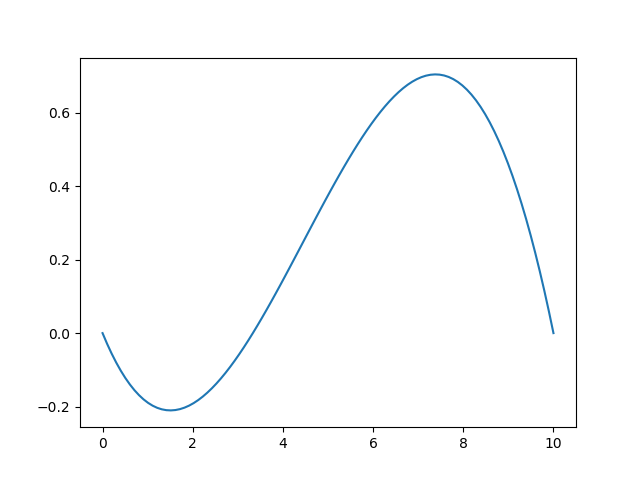
\includegraphics[scale=0.5]{polynominal.png}
        \caption{$\varphi(x)$ for the parameter setting $a=5, b=3, c=0, d=2$}
\end{figure}
For the purpose of analyzing the properties of the replicator dynamic, it is 
useful to introduce some volcabulary used in dynamical system theory. 

A solution through an initial state $x_0$ of the dynamical system is called a 
\textit{trajectory}, whereby it is distinguished between a forward trajectory 
for $t \rightarrow \infty$ and backward trajectory for $t \leftarrow \infty$.
Analytical solutions, i.e. a solution one can express with the use of
basic functions, can only be derived for simple cases. 
It is easier to solve the differential equation numerically using some
computer software. 
However, the existence and uniqueness of a solution through
any initial state for the replicator dynamic is guaranteed by the theorem 
of \textit{Picard-Lindel\"of}, theorem 6.1 in 
\textcite[74]{weibull_evolutionary_1997}. 

The natural question that arises once a solution is obtained, is whether there 
is a connection between the evolutionary dynamic and the equilibria in the 
stage game. To see this, consider the concept of a fixed point.
A point $x^* \in \realnumb^2$ of a dynamic system, such as the replicator 
dynamic in \eqref{eq:replicator}, is called a fixed point
if $\dot{x}(t) = \varphi(x^*) = 0$ i.e. it stays in the current state for all 
$t \rightarrow + \infty $. 
Analyzing \eqref{eq:replicatorpara}, this happens if either a strategy
is not present in the population or the excess payoff of a strategy is zero. 
In the stag hunt game, the fixed points of the
dynamic coincide with the Nash equilibriums of the stage game, 
$\varphi(x^*) = 0$ for $x^* \in \{0,\frac{\alpha_2}{\alpha_1+\alpha_2},1\}$. 
It suffices to calculate the roots of the polynominal $\varphi(x)$, either
numerical or, as the Nash equilibria are usually calculated beforehand,
reducing the degree by polynominal division. In general, the replicator 
dynamic lacks the \textit{Nash stationarity} property and hence there are 
games with fixed points which are not Nash\footnote{For a trivial example, 
consider the prisoners dilemma in \ref{fig:pd}. A population only consisting of 
cooperating agents stays in that state, which is not a Nash equilibrium even 
though it is Pareto-dominating.} \parencite{sandholm_population_2010}.
Concerning fixed points, one is usually interested if the fixed points of 
a dynamic system are stable in terms of some disturbance of the system. 
There are different approaches to stability. A quite strict and useful one 
in the stag hunt game is \textit{asymptotic stability}. 
It essentially requires that a system in a specific fixed point returns 
to the fixed point after a perturbation happened.
Hence, the system tends to move back to an asymptotically stable fixed point
once disturbed. Formally, a $\epsilon$-perturbation of 
\eqref{eq:replicatorpara} is a trajectory of the system with the initial
condition $x_0$ at some ball $B_\epsilon(x)$ of radius $\epsilon >0$ and 
$x_0 \neq x^*$. The fixed point $x^*$ is then called \textit{asymptotically
stable} if there exists an $\epsilon$-perturbation for that $x(t) \rightarrow
x^*$ as $t \rightarrow \infty$. 
The \textit{basin of attraction} of a fixed point $x^*$ is defined as the set 
of points $x_0 \in \realnumb$ for which a trajectory through $x_0$ approaches 
the fixed points $x^*$. In the one dimensional case, this is simply the range 
of $x$ for that any solution to the differential equation with the inital 
conditions in this range converges to the fixed point. With the following 
theorem independently contributed by \cite{hartman_lemma_1960} and 
\cite{grobman_homeomorphism_1959}, one can easily 
find the asymptotically stable fixed points in the stag hunt game:
\begin{mydef}
        If a one-dimensional dynamical system $\dot{x}(t) = \varphi{x}$ 
        has a hyperbolic fixed point $x^*$, $x^*$ is asymptotically stable
        if its linearization 
        $\dot{x}(t) = \frac{\partial\varphi(x)}{\partial x} := \varphi'(x)$ 
        is asymptotically stable. 
        A fixed point is called hyperbolic in one-dimension if 
        $\varphi'(x^*) \neq 0$ and the linearization is stable at that
        point if $\varphi'(x^*) < 0$.
\end{mydef}
The solution to the linearization can be analytical derived by 
a standard tool for differential equation - seperation of variables and 
intergration.
The linearization around the fixed point $x^*$ is accordingly
$x(t)= x(0) e^{\varphi'(x^*)t}$, where $x(0)$ denotes the 
initial condition, i.e. the share of agents choosing strategy 1 in the 
beginning.
Applying the theorem to \eqref{eq:replicatorpara}, one finds that the 
fixed point $x=0$ corresponding to the Nash equilibrium of hunting hare, is 
asymptotically stable, since $\varphi'(0) = - \alpha_2 <0$. 
The linearization around the fixed poin is $x(t) = x(0) e^{-\alpha_2 t}$, 
which clearly approaches zero as $t \rightarrow \infty$. 
Similiarly, the Nash equilibrium 
of hunting stag at $x=1$ is a asymptotically stable fixed point as
$\varphi'(1) = -\alpha_1 <0$ with linearization $x(t) = x(0) e^{-\alpha_1 t}$.
However, the linearization theorem cannot be used for the mixed Nash 
equilibrium, hence the dynamical system is not hyperbolic there, 
$\varphi'(\frac{\alpha_2}{\alpha_1+\alpha_2}) = 0$. Nevertheless, suppose 
there is some $\epsilon$-perturbation of the system  \todo{Voooodoooo}
 with $x_0= \frac{\alpha_2}{\alpha_1+\alpha_2}+ \epsilon$ and 
 $\frac{\alpha_1}{\alpha_1+\alpha_2} > \epsilon > 0$. Plugging this into
 \eqref{eq:replicatorpara} one sees that $\dot{x} >0$, the population share
 grows monotonically for every $\epsilon$, converging to the fixed point 
 $x = 1$. Conversely, for $0 > \epsilon > \frac{\alpha_2}{\alpha_1+\alpha_2}$,
 $\dot{x} < 0$ and so the population share of agents 
 playing strategy 1 decreases monototically, until it reaches the 
 fixed point $x=0$. This is also shown in figure \ref{fig:basinofattraction}.
 \todo{Better description of the graphic}
 The horizonal line marks the mixed-strategy fixed point at $75\%$ for the
 parameter setting $\alpha_1 = 1$ and $\alpha_2=3$. If the population starts
 at this fixed point it by definiton stays there without any disturbance. 
 But any invasion of individuals with a uniform strategy leads away from
 this fixed point, resulting in convergence to one of pure strategy equilibria.
 The use of the word invasion is not by coincidence. It clearly shows the 
 connection of the evolutionary stable strategy of the stage game to the 
 stable fixed points of the dynamic. In fact, one can prove that this is not
 only true in the simple stag hunt, but it holds also under general settings.
 \todo{Folk theorem of evolutionary game theory}
\begin{figure}
        \centering
        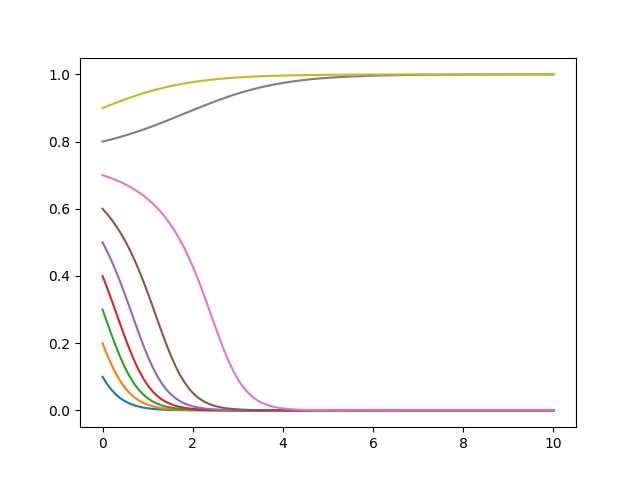
\includegraphics[scale=0.5]{basinofattraction.png}
        \caption{Replicator dynamics in the stag hunt game for 
                $\alpha_1=1,\ \alpha_2=3$ with different initial conditions}
                \label{fig:basinofattraction}
\end{figure}

Concering the equilibrium selection, the evolutionary approach with replicator
dynamic has a definite answer. The population will reach one of the three
Nash equilibria depending on the initial condition. 
However, an equilibrium not asymptotically stable is rather unplausible,
because it only emerges from one initial condition, where the population
is already exactly in that population state. 
Intuitively, one addtional agent playing
a pure strategy suffices to get the population state moving to one of the
pure equilibria. As the model outlined here is only a deterministic
approximation, any stochastic shock would lead to such a disturbance and hence
would start convergence to one of the states with evolutionary stable 
strategies.
The population converges to the stag hunting or the hare
hunting equilibrium if the inital conditions lie in their basin of attraction.
As discussed, the population converges to the state $x=1$, the stag hunting 
equilibrium of the stage game, for all inital conditions 
$x_0 \in (\frac{\alpha_2}{\alpha_1+\alpha_2},1]$. Any trajectory of the 
dynamical system with initial conditions 
$x_0 \in [0,\frac{\alpha_2}{\alpha_1+\alpha_2})$ lead to the hare hunting
equilibrium. Interestingly, one observes another connection of the 
dynamic with the stage game. The basin of attraction is larger for the
risk-dominanting equilibrium. By definition \eqref{eq:riskdom}, 
the hare hunting equilibrium risk-dominates if $\alpha_2 > \alpha_1$,
so in fact the basin of attraction is larger. With the parameter setting shown
in figure \ref{fig:basinofattraction},$75\%$ of the possible initital 
conditions lead to the risk-dominant equilibrium, whereas only $25\%$ of the 
initial conditions lead to the payoff-dominant equilibrium. 
The equilibrium selection is determined by the position of the initial
condition. However, it is not clear what specifies the initial conditions. 
If for example the agents choose a random strategy in a first round of the 
game, independently of each other, one can say that the equilibrium with the
larger basin of attraction, the risk-dominant equilibrium, is more likely 
reached. \todo{what does evolutionary game theory tell about inital condition} 
Giving an exact answer which equilibrium will be selected through the dynamic
process, this approach still leaves us with the problem of what agents 
choose in a first round one-shot game. Section \ref{sec:empiricalevidence} 
summarizes evidence found in laboratory stag hunt game concerning the 
one-shot game strategy choice and so the justification for initial conditions.

\section{A simple model of project coordination}
Outlining a model of coordination among students choosing software for their
assignments, this section tries to investigate the effect of a network 
externality accompanied with a strategy in a evolutionary setting.

In unversity, students are faced with assignments and projects, which are 
often performed in groups with fellow students.
Nowadays, most of them involve some kind of software tool to either present 
the results, analyze the subject or just manage the process of aggretating 
knowledge. Usually the choice of the tools can be simplified to two 
possibilities. One can either use proprietary software
which is usually more user-friendly, but costly due to relative high 
license cost for either the student or the institution using it. 
Beyond that, students can choose to use open source software which is freely
available and can be customized, contrary to proprietary software,
for the personal needs. 
For simplifaction, I assume that during their studies, a larger body of 
students is randomly paired into groups of two playing a coordination game
in which they have two strategies available. In that game both contribute 
to their group project independently, using either open source software, 
represented by strategy 1 or proprietary software, i.e. strategy 2.
If both players choose strategy 1, both use open source software receiving 
the utility $a$. Players that fail to coordinate on the same type of
software, the player using proprietary software receives the utility $c$ and
the player contributing with open source software gets $b$. I assume that 
for the utilities $a>c>b$ holds, 
as they benefit from coordination to open source,
because of the high customizability to their project. The "costs" of 
miscoordination are beared by the student using open source, because he has
to port \footnote{In practice, it is
often easier (and so wanted by producers of proprietary software) to
transform from open source to closed source than the other way due to the
portability.} his results to the proprietary standard, hence receiving only
$b < c$. The last strategy pair is coordination on proprietary software where
both receive the payoff $d$. High cost for licenses despite the success 
in coordination, I assume that $a>c\geq d>b$. So, by assumption, the students
play a stag hunt game as shown in figure \ref{sh}.
Therefore, the analysis of the previous section hold. Coordination on open
source software is the payoff-dominant Nash equilibrium, but it is 
risk-dominant to coordinate on proprietary software. 
The students are not fixed to one other student in their study life and
meet other students they have to do a project with, randomly assigned by their
professor. Additionally, I assume that they are not perfectly rational and
do not revaluate their software choice each time they have to do a project. 
For simplifaction, students
in this model behave according to the revision protocol of pairwise
proportional imitation discussed in section \ref{sec:revisionprotocols}. This
is justified, because most students actually tend to use the software they
always used except when they go to know some other students telling them about
another software they were productive with in their last project. So, 
every once in a while a student gets to know another student and then he switches
away from his software choice following the revision protocol. 
Therefore the dynamic in the model can be described by the replicator dynamic
derived for the stag hunt game in equation \eqref{eq:replicatorpara}.
This model would not differ in terms of convergence and stability of Nash 
equilibria to the evolutionary stag hunt game above.

However, I want to introduce "network externalities" in this model. 
The interest of the economic literature turned to open source software 
development, because it is commonly observed that users contribute to 
projects without receiving payment for it.
In fact users share their source code publicly to the open source community,
being motivated by reputation and the signaling effect one can achieve.
The utility for a user then increases with the size of the community as 
more people contributing code increases the variety and usefulness of the 
software. I incorporate that in the model by letting the utility for a student 
in the case of coordination on open source software be a function of 
population size using that strategy, $f(x)$. 
Preserving the general structure of the
game, it is useful to focus on the functional specification 
$f(x) = a + e(x)$, where $a$ is the paramater used previously and $e(x)$ 
denotes the network externality. 
A positive network externality therefore satisifes $e(x)>0$ and 
$\frac{de(x)}{dx}$, an increase of the population share choosing the strategy
also increases the utility due to the network. Including the
parameter $a$ makes sure that the utility of this strategy combination is 
never below the utility of coordination on proprietary software. So to say,
the network externality adds to the fact that open source software is cheaper 
and customizable. The payoff matrix, using local shifts, than is 
$A=\begin{psmallmatrix}\alpha_1+u(x) && 0 \\ 0&& \alpha_2\end{psmallmatrix}$. 
Substituting into the replicator dynamic  \ref{eq:replicatorpara} one gets:
\begin{alignat}{2}
        \dot{x} = \varphi(x) = x^2(\alpha_1+e(x) +2\alpha_2 ) 
        - x^3(\alpha_1+e(x)+\alpha_2) - x(\alpha_2)
        \label{eq:externalitymodel}
\end{alignat}
Plugging $x=0$ and $x=1$ into equation \eqref{eq:externalitymodel} one can 
ensure that the fixed point with pure strategies and their
property of asymptotical stability did not change.
($\varphi'(1) = -\alpha_1 -e(1),\ \varphi'(0) = -\alpha_2 -e(2)$)
In \cite{paperaboutnetworkexternality} a linear form for the network
externality is suggested. With the additional parameter $\beta \in \realnumb_+$
one than gets $e(x) = \beta x$. While not changing the state in which
the whole population coordinated to one strategy, the inner fixed point
is changed by the dynamic. $\varphi(x)$ is still a polynominal but of 
degree $4$:
\begin{align}
        \dot{x} = \varphi(x) = -\beta x^4 -x^3(\alpha_1 + \alpha_2 
        - \beta ) + x^2 (\alpha_1 + 2 \alpha_2) - x(\alpha_2)
\end{align}
Using the knowledge from the general case, we can find the roots, i.e. fixed
points of the dynamic, by reducing the degree with the two roots known. The
polynominal of degree $2$ can then be solved applying a quadratic formula\footnote{
The solution with negative sign was omitted, since it has no economic 
interpretation}, so that the fixed point with a mixed population state is
$x_3 = -\frac{\alpha_1+\alpha_2}{2 \beta} + 
\sqrt{(\frac{\alpha_1+\alpha_2)^2}{4\beta^2} +\frac{\alpha_2}{\beta}}$. 
Some arithmetic can verify that $0<x_3<\frac{\alpha_2}{\alpha_1+\alpha_2}$, 
is in the feasible range of the population share variable. 
Taking the limit, $\lim_{\beta \rightarrow 0} x_3 = 
\frac{\alpha_1}{\alpha_2+\alpha_1}$, approves the intuition that for a 
diminishing network externality the model without externality is obtained.
The plot of the dynamic and the polynominal is 
shown figure \ref{fig:plotmodellinear}.
Note that the share of students choosing strategy 1 is now lower at the 
inner fixed point, showing that the positive externality has a positive 
effect on the attractiveness of choosing open source software. Indeed,
the basin of attraction of the equilibrium in which all students are using 
open source software became larger, depicted by the distance to the
inner fixed point.
Comparison of the dashed, red horizontal line, the inner fixed point without 
externality, with the dashed, green horizontal line, the inner fixed point 
with externality, in figure \ref{fig:dynamiclinear}, illustrates this. 
\begin{figure}[h]
        \centering
        \begin{subfigure}{.5\textwidth}
        \centering
        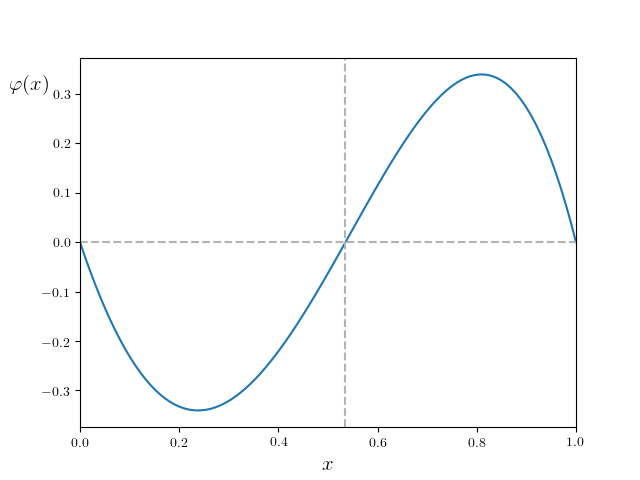
\includegraphics[scale=0.5]{polynominallinearmodel.png}
        \caption{The polynominal with marked roots} 
        \end{subfigure}%    
        \begin{subfigure}{.5\textwidth}
        \centering
        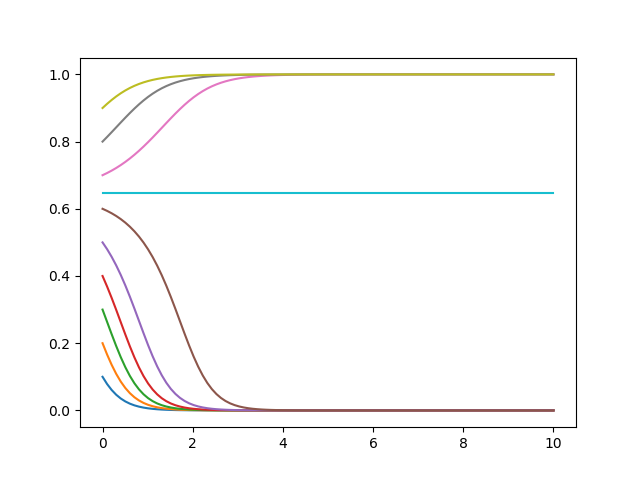
\includegraphics[scale=0.5]{dynamiclinearmodel.png}
        \caption{The dynamic} 
        \label{fig:dynamiclinear}
        \end{subfigure}%        
        \caption{The linear externality model for parameters $\alpha_1=1,\alpha_2=3,
        \beta=3$}
        \label{fig:plotmodellinear}
\end{figure}
The basins of attraction have equal size for $\beta^* = 2 (\alpha_2 -\alpha_1)$,
attracting an equal amount of initial conditions. However,
the proprietary equilibrium looses its risk-dominance property 
only for $1 > x > \frac{\alpha_2-\alpha_1}{\beta}  $, using definition 
\ref{eq:riskdom}. The right hand side of the equation must be lower than one 
to change the risk-dominance property. This leads to the conclusion 
that in this model, the size of the basin of attraction and the risk-dominance
property do not coincide in general, since the externality changes the Nash 
product associated with the pure strategy 1 equilibrium. Consider for example 
the parameter setting $\alpha_1 =1, \alpha_2=3$, but now let $\beta=3$. 
The basin of attraction is not equal, since $3<\beta^*= 4$. 
The open source equilibrium attracts all trajectories starting within 
$x_0 \in (\frac{-2+\sqrt{13}}{3},1]$ and hence the propriertary equilibrium attracts
all trajectories $x_0 \in [0,\frac{-2+\sqrt{13}}{3})$. Clearly, the latter basin of 
attraction is larger ($\frac{-2+\sqrt{13}}{3}>0.5)$, 
but the open source equilibrium gets risk-dominant for
$x>\frac 23$. Implying that the network externality not only increases the
utility obtained from the choice of open source software, but also,
combined with a high enough user base, makes this choice risk-dominant.

The model presented here is quite a simplification of the real world. 
First, the students are expected to be able to review which software is 
appropriate for their projects, hence have more information available then 
assumed in the model. Secondly, talking to their fellow student seems
possible before deciding which software to use for the project. 
However, as the experimental literature, discussed in 
\ref{sec:experimentalevidence}, and \textcite{aumann_nash_1990} suggests, 
cheap talk does not generally solve the coordination problem. 
Additionally, the way the attractiveness of a strategy increases with
the population size, the network externality, is modeled quite naive.
Students in university, and social networks in general, are not fully
connected, as students, for example, only do projects with fellow students
in the same classes. Furthermore, students usually try to do projects
with people they are socially connected with. In fact, the assumption about
a fully connected network is "one of the main criticisms of evolutionary game
theory" \parencite{hanauske_evolutionare_2011}. As a consequence, many
researchers recently gave attention to the structure of the network underlying
the interaction of agents and the evolving of this structure 
\parencite[46]{szabo_evolutionary_2007-1}.
For example \textcite{ohtsuki_simple_2006-1} found, that fewer connectivity 
leads to more cooperation, because "The fewer friends I have the more strongly 
my fate is bound to theirs" \parencite[1]{ohtsuki_simple_2006-1}.
Although the model with a positive linear network externality is far to simple 
to capture the effect of complex, adapting networks, it gives an intuition of 
how coordination of a small group, in this case two players, is affected by 
the choice of the whole population.





\section{Experimental Evidence}
\label{sec:experimentalevidence}
A third approach beside the traditional and the evolutionary treatment of 
coordination problems is what \textcite{camerer_behavioral_2003} calls the 
'fundamental empirical' approach.
Hence, this section surveys the experimental economic literature regarding 
laboratory coordination games to provide evidence how actual people choose
their strategies in such situations and which factors might influence them. 
Precisely, do people, if they are able to coordinate on an equilibrium at all,
play the risk-dominant or the payoff-dominant equilibrium? And how does their
choice change playing the game repeatedly?
Due to the rich experimental literature on coordination in social 
dilemmas, the focus will be on studies with a similiar framework as the
evolutionary SH game. A comparison will show the shortcomings and what
is described well by the evolutionary framework.
 
Due to the different notations authors use, a translation into the present
notation was performed.
On these grounds, the 
strategy used in the payoff-dominant equilibrium of the SH game will be 
either called  \textit{strategy 1} or in analogy to the stag hunt story 
\textit{hunting stag}.
Consistently, the strategy used in the risk-dominant equilibrium is called
\textit{strategy 2} or \textit{hunting hare}. 

The papers of \textcite{van_huyck_tacit_1990} and 
\textcite{cooper_communication_1992} are seen as the first experiments 
investigating coordination games \parencite{devetag_when_2007}.
In \textcite{van_huyck_tacit_1990}, subjects do not play a stag
hunt, but an order-statistics game. These games differ in that subjects can
choose from a broader set of strategies and hence there are more than two 
equilibria in the game. The games are played in a group and the payoff to 
all players depend on the lowest strategy one of them chose, thus the name 
'weak-link' order statistics game. Nevertheless, the structure is similiar to
the stag hunt in the way that the equilibria are Pareto-ranked, with one 
'safe' strategy \parencite{devetag_when_2007}.
So evidence from this games is 
likely to be transferable to the coordination problem in the stag hunt game. 
In \cite{van_huyck_tacit_1990} subjects played the order-statistics game in 
groups of 14-16 for 10 periods. They only received information about their 
payoff, but so they could find out what the lowest choice of one subject in 
their group was. Astonishingly, in every experiment the groups converged
to the equilibrium with the lowest payoff. 
This result were preserved in another 
five periods of this game although the subjects played an alternative payoff
matrix embracing the payoff-efficient equilibrium across all groups 
inbetween. 
Replications of this results have been performed numerously, with 
varying group sizes and slightly changed payoff matrices. 
One may consult \textcite{devetag_when_2007} for a summary. 
\todo{Summary or not?}
\textcite{cooper_communication_1992} perform a experiment with a standard 
two-player stag hunt game\footnote{They call 
it simple coordination game(SCG).} 
and one augmented by a dominated strategy. They find that 
subjects in randomly matched one-shot games, knowing only about their own
received payoffs, also fail to coordinate without any preplay communication. 
However, they find that two-way communication, in which both players were
able to send a message to their matched partner containing which strategy
they intend to choose, solves the coordination problem in the SCG. 
This early approaches suggest that coordination failure\footnote{Here in the 
meaning of not being able to coordinate on the payoff-dominant equilibrium} 
is common in laboratory \parencite{devetag_when_2007}. 
It is noteworthy that the studies 
discussed use different matching protocols, fixed matching in groups and 
random matching against one other player, and yet found the same results. 
As a consequence, experimentalist focused mainly on the characteristics 
of the payoff matrix instead of implementational details in laboratory SH 
games.
\parencite{devetag_when_2007}.

The implementation of random matching in a group is closest to the 
evolutionary setting discussed in section \ref{evolutionarysection}, because
there a group of player, repeatedly matched in pairs, play the stag hunt 
game, having only information about their own payoff and the payoff their
opponents used. Certainly, it is to suspect that real players, opposed
to the programmed agents in the evoltuionary setting, are able to remember
what the other players chose in the rounds before. \todo{historyofplay}
Random matching was conducted by \textcite{battalio_optimization_2001}. 
Subjects played three stag hunt games with the typical symmetric pure strategy
equilbrium and the symmetric mixed strategy equilibrium at $(0.8,0.2) \in
\Delta$. Figure \ref{payoffbattalio} shows the payoff matrices of the
games $2R, R$ and $0.6R$ used. The names become clear when observing the 
\textit{optimization premium} of the games. While controlling for the basin of 
attraction of the equilibria - the mixed equilibrium is equal in all games -
they want to explore the effect of an increase in the "premium for playing
a best-response" \parencite[751]{battalio_optimization_2001}. 
In order to investigate this, they define the optimization premium $r_j(y)$ of 
a game $j$ as the difference in payoffs choosing the pure strategies 
$e_1$ and $e_2$ while expecting the opponent to play a strategy 
$y=(q,1-q) \in \Delta$:
\begin{align}
        r_j(y)= \hat{F_j}(e_1,y) - \hat{F_j}(e_2,y) = \delta_j(q-q^*),
\end{align}
with the \textit{optimization premium parameter} $\delta_j$. In the notation
parametrized SH game, $\delta_j = a - c + d - b$.
The parameters for the payoff matrices are reported in figure 
\ref{payoffbattalio}. 
First of all, they find support for their hyptohesis that in games with a 
larger optimization premium subjects coordinate less frequently on the 
payoff-dominant equilibrium. 
Contrary to game $0.6R$, where only one cohort coordinated according 
to risk-dominance, in $2R$ no cohort and in $R$ only one cohort 
converged to the payoff-dominant equilibrium. The replicator dynamic does 
not offer a description of this behavior, since convergence to an 
equilibrium only depends on its basin of attraction once the dynamic 
started, which do not differ for the three games. 
Whereas "all 24 cohorts start in the basin of attraction
of the risk-dominant equilibrium" \parencite{battalio_optimization_2001}, 
all should converge to the risk-dominant equilibrium according to the dynamic.
In most cases this is true, with only three exceptions in game $0.6R$ 
and two in $R$.
But, for the sake of completness, a crossing of the  
"best-response separatrix" \parencite{battalio_optimization_2001} i.e. 
mixed-strategy equilibrium, can not happen in the deterministic replicator 
dynamic.
Furthermore, as they conjectured, a larger
optimization premium increases the speed of convergence. Hence, a coordination
on a equilibrium was achieved fastest in the $2R$ game. 
This is consistend with a postulated replicator dynamic for this games. 
Starting from \eqref{eq:replicator}, one can derive that the dynamics of this 
games are the same up to a change in speed, proportional to the ratio of 
optimization premia of the games. In game $R$ the change in the population share
playing strategy one is, thus, half the speed of $2R$ and four thirds of $0.6R$,
$\dot{x}_{R} = \frac 12 \dot{x}_{2R} = \frac{4}{3}\dot{x}_R$.

\textcite{schmidt_playing_2003} designed their experiment such that the effect
of differing risk levels could be observed. It is convenient to relabel 
the strategies in the game, because in their treatment the payoff-dominant 
equilibria is in the right corner of the normal form game representation,
contrary to the notation used throuhout this text. Comparing risk levels between
games, they used a measure due to \textcite{selten_axiomatic_1995}, defined
as:
\begin{align}
        \label{riskmeasureschmidt}
        R = ln\left(\frac{\hat{F}(e_2,e_2) -\hat{F}(e_2,e_1)}{\hat{F}(e_1,e_1) 
        -\hat{F}(e_2,e_1)}\right) = ln \left(\frac{d-b}{a-c}\right).
\end{align}
The risk measure $R$ is positive, if the Nash equilibrium $(e_2,e_2)$ is
risk-dominant, and negative if the payoff-dominant equilibrium inhibits both
properties.
None of the four games in \textcite{schmidt_playing_2003} handles
the case of $R=0$, where the mixed-strategy equilibrium is risk-dominant.
In difference to \textcite{battalio_optimization_2001}, they do not
use the proposed optimization premium, but rather measure the risk-dominance 
level in relative terms as $P=\frac{a-d}{a}$.\footnote{As they mention, the 
games in \textcite{battalio_optimization_2001} vary in their level of 
P accordingly.}
The payoff matrices of the games are shown in \ref{fig:payoffschmidt}.
Comparing Game 2 with Game 3, and Game 1 with Game 4, the only difference is the 
degree of risk-dominance and hence one can investigate if subjects react 
to the change in risk-dominance. For game 1 and game 3 the basin of attraction
of both equilibria is equal (Mixed-NE at $(\frac 12, \frac 12)$) and  for
game 2 and 3 the Mixed-NE is at $(\frac 34,\frac 14)$ resulting in the typical 
larger basin of attraction of the strategy $(e_2,e_2)$. Therefore, it is  
expected from the replicator dynamic, of course depending on the inital condition 
of the game, that subjetcs are more likely attracted to the 'hare-hunting' 
equilibrium in game 2 and 3.
\textcite{schmidt_playing_2003} implement three different types of matching
protocol. First of all, a random matching protocol where each subject is not
matched twice with another person and only has information about his payoff and
the action of the person he was matched against. 
Secondly, a fixed protocol, matching two persons for several rounds against 
each other, followed by a series of one-shot games. 
In the random matching protcol, they find evidence that an increase in 
risk-dominance, i.e. an increase in $R$, leads to a higher choice of the
strategy in the risk-dominant NE.\todo{Schmidt et al paper.} 

\textcite{dubois_optimization_2012} conducted a similiar experiment as 
\textcite{schmidt_playing_2003} and \textcite{battalio_optimization_2001},
but introduced a different measure for the risk subjects are confronted with in
the games. They defined the \textit{relative riskiness} of a games 
"safe strategy relative to the risky strategy" as $RR = \frac{|c-d|}{a-b}$. 
\todo{Hier Zitation?}
Intuitively, a player commited to strategy one and calculating the 
difference a deviation of the other player from strategy one to two, gets
$(a-b)$. Similiary for strategy two, he receives $(c-d)$. The relative riskiness
measure is, hence, the ratio of the effect a deviation of the other play has 
on the payoff. Alternatively, it can be interpreted as the ratio of the 
standard deviations of the payoffs \parencite{dubois_optimization_2012}. 
They speak of "comparable riskiness", if the $RR$ measure is close to one 
\parencite[372]{dubois_optimization_2012}. 
According to $RR$, the risk-dominant 
strategy 2 is said to be less risky relative to the payoff-dominant strategy 
one in on game compared to another if the $RR$ is smaller.
Observing the values of the relative riskiness by 
\textcite{dubois_optimization_2012} and the risk-dominance measure of 
\textcite{schmidt_playing_2003} for the games used in the papers, it is clear
that both measures are in a conflict. As by \textcite{schmidt_playing_2003}
\todo{possessivcite}
measure, risk-dominance is kept constant in the games of 
\textcite{battalio_optimization_2001}, whereas relative riskiness indicates a
variation. On the other hand, relative riskiness cannot distinguish between
the games 1,2 and 3 of \textcite{schmidt_playing_2003}, since $RR=0$. In an
early working version of their paper they explicitly excluded the case 
$c \neq d$ and statet that "a more general measure of relative riskiness 
should allow for the case where c=d as compared to $(a-b)$ 
\parencite{dubois_optimization_2008_working}. 
\todo{Maybe both measures capture different things: Intuition}
Game 1 replicated \textcite{battalio_optimization_2001}'s 
game\footnote{The payoff matrices are identical} $0.6R$. 
Compare \ref{fig:payoffdubois} and \ref{fig:payoffbattalio}}. 
As per their conjecture, they found that a lower relative riskiness 
in a game decreases the rate strategy one was chosen, 
keeping the optimization premium constant. This is congruent with 
the intuition that the severity of the impact related with the 
strategic uncertainty subjects face in a game, expressed in
the difference in payoff a deviation of the other player would cause,
effects the choice of the strategy. 
On the other hand, keeping the relative riskiness constant and varying the
optimization premium, they cannot find an effect on the frequency of 
strategy 1. 
In measuring the "coordination sucess", they deploy the concept of "strong
coordination". 
In other words, counting the occurence of periods in which a group
uniformly adopts a strategy such that every pair of subjects lands in one
of the Nash equilibria. \textcite{dubois_optimization_2012} intend to sort 
out "furtuitous coordination", coordination as consequence of subjects being
randomly matched with each other \parencite[373]{dubois_optimization_2012}.
Comparing strong coordinations between the games they find a non-significant 
difference between game 1 and game 2 in which only the relative riskiness 
ceteris paribus was changed. Contrary to that, there is a significant 
difference in the commonness in game 3 to game 2.
Since game 3 and 2 only differ in their optimization premium, 
\textcite{dubois_optimization_2012} conclude that a higher optimization
premium leads to more frequent (strong) coordination. 
As they mention, this agrees with the observation of 
\textcite{battalio_optimization_2001} that the speed of convergence depends 
positively on the optimization premium. 
\todo{Is it really the convergence or did I miss something?}
\todo{History of Play}

As seen from the evidence \textcite{battalio_optimization_2001},
\textcite{schmidt_playing_2003} and \textcite{dubois_optimization_2012} 
found, the structure of the payoff matrix has a strong impact on the way 
people play the stag hunt game.   
The story this evidence tells is quite frightening. Failure to coordinate 
on the payoff-dominant equilibrium seems to be common. 
Following an argument of \textcite{kreps_game_1990} that identical strategic 
interactions, such as the play of completely indentical stag hunt games 
in the laboratory, "take us very little distance outside the laboratory" 
\parencite[212]{kreps_game_1990}, 
\textcite{rankin_strategic_2000} design an experiment with a randomly 
pertubated stag hunt game. Essentially, the payoff to strategy 1 is fixed 
whereas the payoff to strategy 2 varies randomly between the games. This is
depicted in the payoff matrix \eqref{eq:payoffrankin}.
\begin{align}
        \label{eq:payoffrankin}
        A = \mqty(1 & 0 \\ x & x)
\end{align}        
The parameter $x$ is equally distributed between $(0,1)$ and once a sequence
was calculated used for all cohorts participating in the experiment. This
variation justifies to describe the games as "similiar" but not
"identical", hence the structure stays the same, but the risk-dominance 
property varies. Indeed, if $x$ is greater than $0.5$ risk-dominance and
payoff-dominance select different equilibria, $(e_2,e_2)$ and $(e_1,e_1)$,
respectively. For a value of $x$ smaller than $0.5$ both select 
the equilibrium in strategy 1. One finds that the optimization premium for 
this randomly perturbed games does not change, since $\delta=1-x+x+0=1$. 
The relative riskiness measure $RR$ cannot discriminate between this games,
since $|d-c|=0\ \forall x$. \textcite{schmidt_playing_2003} measure of risk of 
course is positive for $x > 0.5$ and negative for $x <0.5$. 
\todo{how to cite?}
The question \textcite{rankin_strategic_2000}
want to investigate is, if this framework of sligthly varied situations may
lead the groups to form a "convention" which deductive principle to choose. 
In contrast to the studies performed with identical stag hunt games, they 
observe coordination to the payoff dominant equilibrium across
all cohorts. Whereas in the first ten periods of play risk dominance seems
to have some explanatory power for the choice of strategy, in the last ten
rounds 91\% choose the payoff dominant action. 
In the cases of coinciding equilibrium selection of risk-dominance and 
payoff-dominance ($x < 0.5$) all subjects coordinated on that equilibrium in 
group 1-5 and 95\% of the subjects in group 6. But also for the other case a 
high coordination on the payoff-dominant strategy was observed, ranging from 
80\% to 95\% of the strategies played, suggesting that there is clear evidence
for the hypothesis of an emerging convention based on the deductive principle
payoff-dominance. This sends a quite positive image about coordination, because 
this is "dramatically at odds with claims that coordination failure is common"
\parencite[9]{devetag_when_2007}. 
As outlined, most studies concerned with the stag hunt game in the 
laboratory focused on the payoff matrix. However, implementational details 
such as the matching protocol influence behaviour sharply. Not only 
\textcite{van_huyck_tacit_1990} found in their two-player fixed matching
convergence to the payoff-dominant equilibrium, 
\textcite{clark_repetition_2001} also found different strategy 
choices between randomly matched one-shot games and fixed matching protocol 
games. The latter lead to significantly higher choices of the strategy 
in the efficient equilibrium and less "disequilibrium play" in general. 
\textcite{devetag_when_2007} mention that one-shot games imply a 
random matching protocol. But it is different to random matching on group
basis, where subjects can play against the same opponent again 
and hence there is the possibility that a "convention" emerges like in 
\textcite{rankin_strategic_2000}.

Even more subtle experiment design differences are conjectured to have an
effect. For example \textcite{devetag_when_2007} suggest that the formulation
"you will remain grouped with the same seven other participants for the next
75 rounds" in the instruction of the \textcite{rankin_strategic_2000}  
\todo{how to cite this}
experiment may increased trust within the group and hence was a 
cause for the exceptional coordination success. Comparatively, the 
instructions in \textcite{dubois_optimization_2012} read "At the beginning
of each period, in each group (composed of 8 participants), the computer
system will form 4 pairs of subjects. [...] The experiment 
involves 75 rounds"\parencite[378]{dubois_optimization_2012}. 
While essentially containing the same information,
it does not emphasize the fact that subjects can reencounter the same 
players again and consequently might have influenced the subjects to play
the strategy associated with less risk.

An interesting experimental approach is executed by 
\textcite{dufwenberg_gender_2005}. They tried to evaluate whether 
there is a difference in coordination behavior accross genders, motivated by 
the different treatment of males and females in the work place. Playing the 
weak-link order statistics game in \cite{van_huyck_tacit_1990}, groups of 
only females or only males face the coordination problem with Pareto-ranked 
equilibria. The motivation of observing gender differences was 
"never explicitly pointed  out to the subjects" 
\parencite{dufwenberg_gender_2005}\footnote{
Even though it might be interesting to see if there is an effect like 
the discussed "crab basket" effect which leads woman to mistrust each other 
more than in a mixed group.} However, they did not find that the groups play
different. Differences in the beginning "disappear fast and no difference
is found in later stages" \parencite[235]{dufwenberg_gender_2005}. 
All groups converge to the choice of the minimum
contribution. As they mention, it might be useful to investigate differences
with groups that also have some other characteristica in common. They refer
to the differences group identity has for females and males playing a 
public goods game. Namely, \textcite{croson_groups_2008} found that when
females in a sorrority play the public goods games they perform better than 
females with no specific belongingness. Contrarly, males in a fraternity 
performed worse than males without a group identity. 
Interestingly, this and other factors concerning the group of subjects 
playing the coordination game might be a rationale for the initial conditions
in the evolutionary dynamic. The intitial conditions might be used to 
capture the composition of the subjects interacting in reflecting how well
trust or cultural convecntions are embedded in the population. 
Nevertheless, it seems difficult, atleast for the author, to justify
the reduction of the inheritance of cultural values to one\footnote{Of course, 
in games with more than two strategies the initial conditions are represented 
by a vector} dimension such as the initial conditions $x_0$.
\todo{External validity}

The discussion of the laboratory research makes on clear: There is more
to the coordination problem than individuals programmed like a robot 
to a strategy, while being attracted and moved to an equilibrium by a dynamic
in a fully deterministic fashion. But, as a model should, the analysis offers 
a simplification that helps to understand some of the patterns observeable 
when real people interact. \todo{maybenot}
\section{Summary and Outlook}
Stag hunt games do not just have to occur in the literal version Rousseau
described, even though there exists an interesting example provided by 
David A. Nolin and Michale S. Alvard on whale hunting in Lamalera, Indonesia
\parencite{nolin_meat-sharing_2000}.
Actually, many situation in economics contain the coordination of actions
of individuals. 
Indicated in the introduction, usually the prisoner's dilemma is then used
as a framework to analyze why individuals may not be able to coordinate on the 
Pareto-dominant outcome. However, as Camerer
suggests, various situations that "are thought to be a prisoner's dilemma 
are actually a stag hunt game", if the described situation "evokes emotion,
has enough synergy or excludability" 
\parencite[376-377]{camerer_behavioral_2003}. Furthermore, repeated prisoner's
dilemma becomes a stag hunt game when only strategies grim trigger
and always defect are compared. \textcite{blonski_prisoners_2003} show that
this relationship is true for other strategies, considering the discrepancy
between Pareto-dominance and risk-dominance as equilibrium selection criteria 
for a wide range of parameter settings. 
Evolutionary game theory provides a theory in which the selection of an
equilibrium is endogenous once the dynamic is set into operation. Yet, it
does not offer an explanation for the initial conditions, which in fact 
determine on which equilibrium the population coordinates. Likewise, the
assumptions about the connection of individuals, discussed in 
\ref{sec:simplemodel}, the continous population and the way agents
adjust their strategy need to be justified for the given application. 



\section{appendix}
\begin{figure}[h]
\caption{Payoff matrices of games in \textcite{battalio_optimization_2001}}
        \label{figpayoffbattalio}
\begin{alignat*}{3}
        A_{2R} &= \mqty(45 & 0 \\ 35 & 40) \quad & &A_{R} = \mqty(45 & 0 \\ 
        40 & 20) \quad & &A_{0.6R} = \mqty( 45 & 0 \\ 42 & 12) \\
        \delta_{2R} &= 50  \quad & &\ \delta_{R} = 25 \quad & &\ \delta_{0.6R} = 15
\end{alignat*}
\end{figure}
\begin{figure}[H]
\label{fig:payoffschmidt}
\caption{Payoff matrices of the games used in \cite{schmidt_playing_2003}}
\begin{alignat*}{3}
        A_{Game1} = \mqty( 100 & 20 \\ 60 & 60), \quad A_{Game2} 
                               &= \mqty( 100 & 20 \\ 80 & 80), \\ 
        A_{Game3} = \mqty( 100 
             & 60 \\ 80 & 80), \quad A_{Game4} &= \mqty( 100
                             & 0 \\ 80 & 60)
        \end{alignat*}
\end{figure}
\begin{figure}[H]
        \caption{Payoff matrices of the games used
        in \cite{dubois_optimization_2012}}
        \label{fig:payoffdubois}
        \begin{alignat*}{3}     
                A_{Game1} &= \mqty(45 & 0 \\ 42 & 12),
                A_{Game2} &= \mqty(40 & 20 \\37 & 32),
                A_{Game3} &= \mqty(44 & 4 \\ 38 & 28) \\
                RR_{Game1}&= \frac 23, RR_{Game2}&=\frac 14, RR_{Game3}&=
                \frac 14
        \end{alignat*}
\end{figure}
\printbibliography
\end{document}







